\section{Methods}
\subsection{Measuring Glenoid Version}
\label{sec:methods}
\sksglenoid currently implements two 3D methods; the two-plane method described by Ganapathi et al. \cite{PMID:20933439} and the 3D corrected 
Friedman method described by Budge et al. \cite{BUDGE2011577}. \sksglenoid also implements two
2D methods; Friedman's method \cite{PMID:1522089} and the vault method described by Matsumura et al. \cite{PMID:24618285}. Each implementation can be accessed by via a command line application which takes as 
input a file describing the anatomical position of the required landmark points.

\begin{figure}
        \begin{center}
                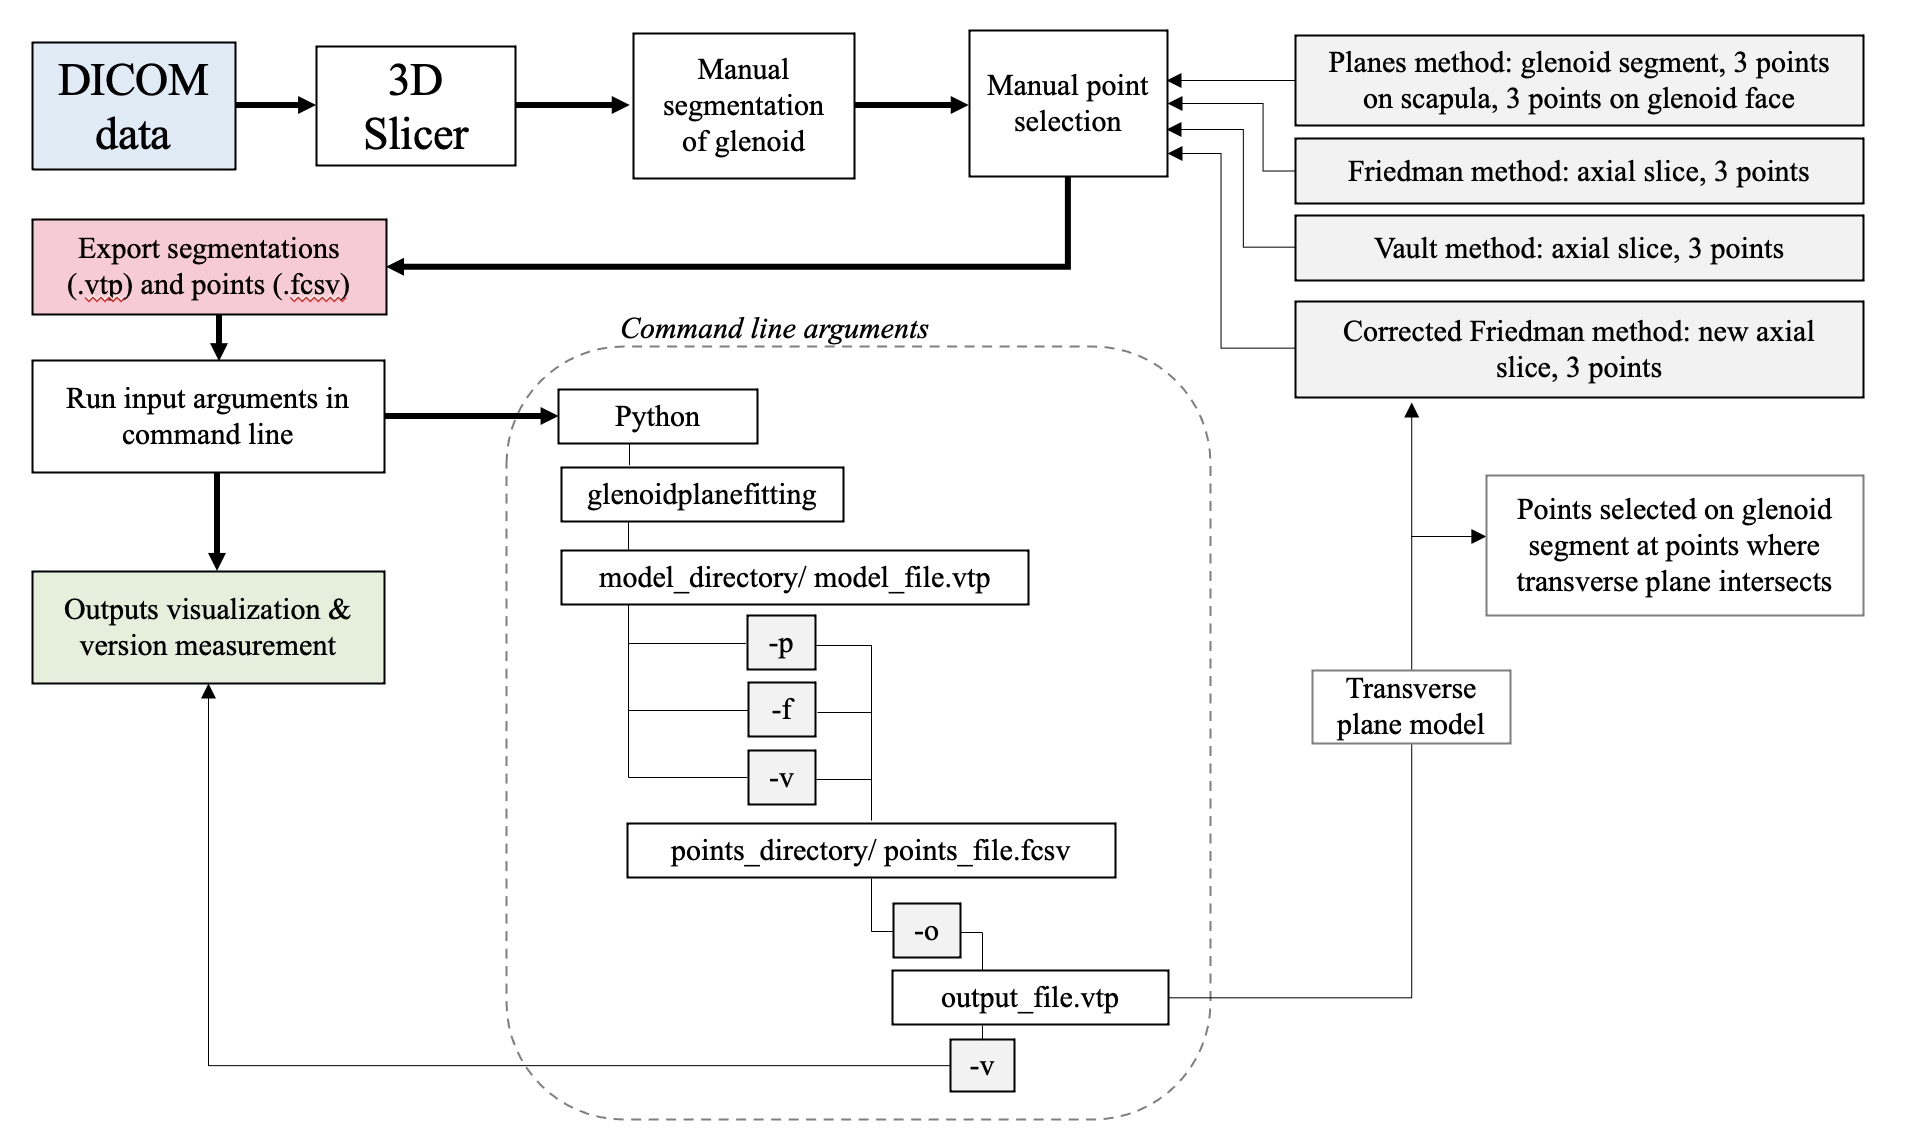
\includegraphics[width=0.98\linewidth]{figures/workflow.png}
                        \caption{\label{fig:workflow}A workflow diagram describing the current workflow. Relevant landmarks 
			are currently identified using 3DSlicer and passed to \sksglenoid via the command line. For the corrected Friedman method the points are manually identified 
			a second time after identification of the new axial slice.}
        \end{center}
\end{figure}

Although the longer term aim is to automate the identification of landmark points, \sksglenoid currently requires the landmark points to be manually identified. 
Figure \ref{fig:workflow} gives a graphical description of the work flow we used. 

The selection of the different landmark points for each method and calculations of version measurements were done as follows. For the two-plane method, 3 points were chosen for each plane. For the glenoid fossa plane the points selected were near the rim, one at the superior pole of the glenoid and two on the lower third of the glenoid anteriorly and posteriorly (black points on figure \ref{fig:visplanes}).  For the scapula plane, the 3 points included one at the center of the glenoid, another at the medial border of the scapula where the scapular spine intersects the scapular body, and a third at the inferior tip of the scapula (orange points on figure \ref{fig:visplanes}). The glenoid version was then calculated as the angle between the plane of the glenoid fossa and the plane of the scapula. 

\begin{figure}
        \begin{center}
                \begin{subfigure}[b]{0.31\linewidth}
			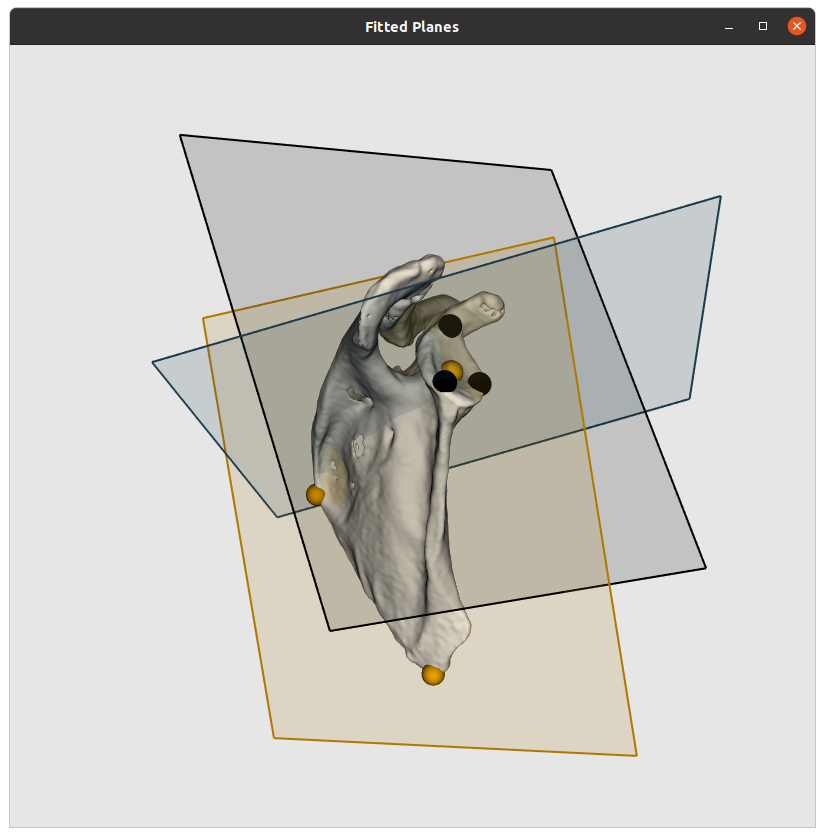
\includegraphics[width=\linewidth]{figures/planes_vis.png}
			\caption{\label{fig:visplanes}Two Plane Method}
		\end{subfigure}	
                \begin{subfigure}[b]{0.28\linewidth}
			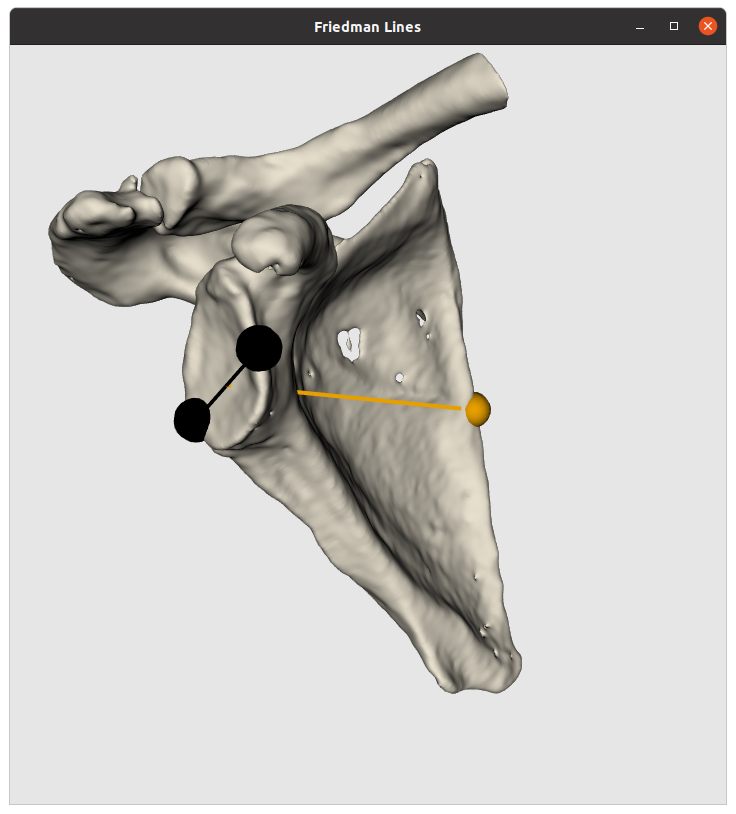
\includegraphics[width=\linewidth]{figures/friedman_vis.png}
			\caption{\label{fig:visfried}Friedman Method}
		\end{subfigure}	
                \begin{subfigure}[b]{0.31\linewidth}
			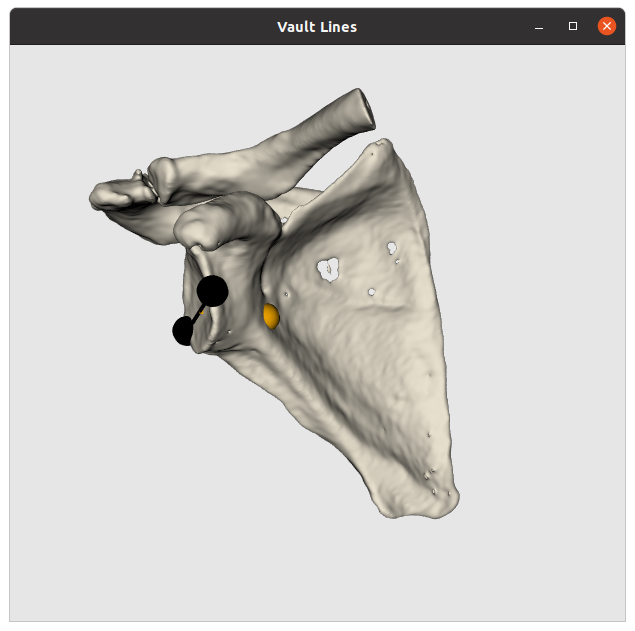
\includegraphics[width=\linewidth]{figures/vault_vis.png}
			\caption{\label{fig:visvault}Vault Method}
		\end{subfigure}	
	\end{center}
	    \begin{center}
                \begin{subfigure}[b]{0.30\linewidth}
			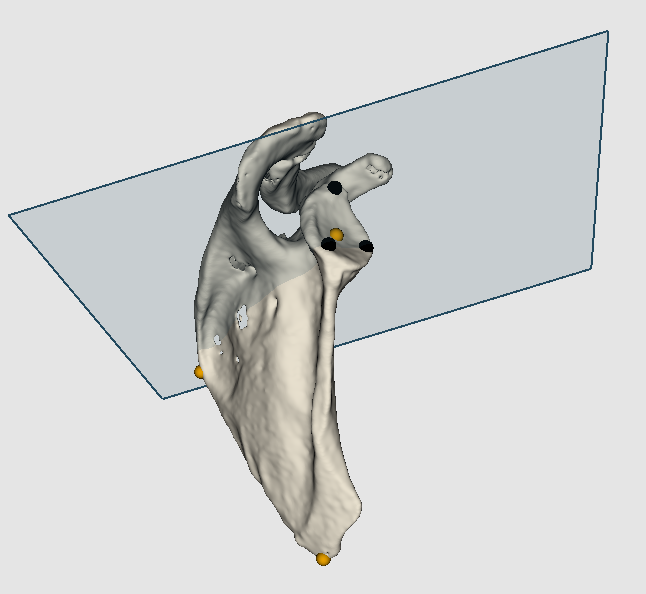
\includegraphics[width=\linewidth]{figures/corr_fried_vis.png}
			\caption{\label{fig:viscorrfried}Corrected Friedman Method}
		\end{subfigure}	
                \begin{subfigure}[b]{0.31\linewidth}
			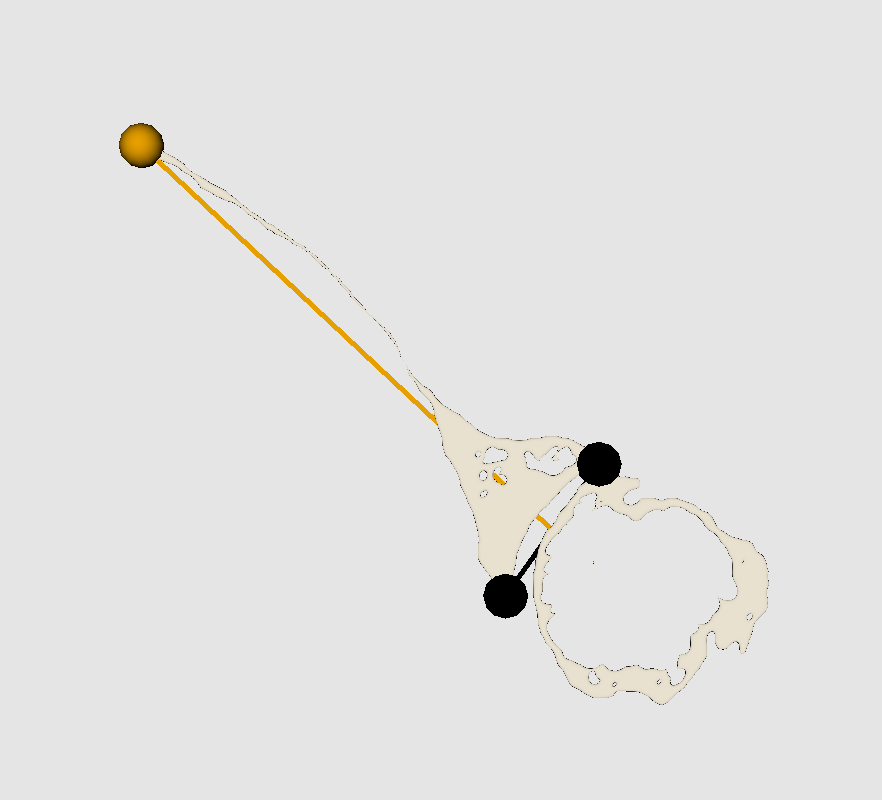
\includegraphics[width=\linewidth]{figures/friedman_vis2D.png}
			\caption{\label{fig:visfried2D}Friedman Method Axial Slice}
		\end{subfigure}	
                \begin{subfigure}[b]{0.31\linewidth}
			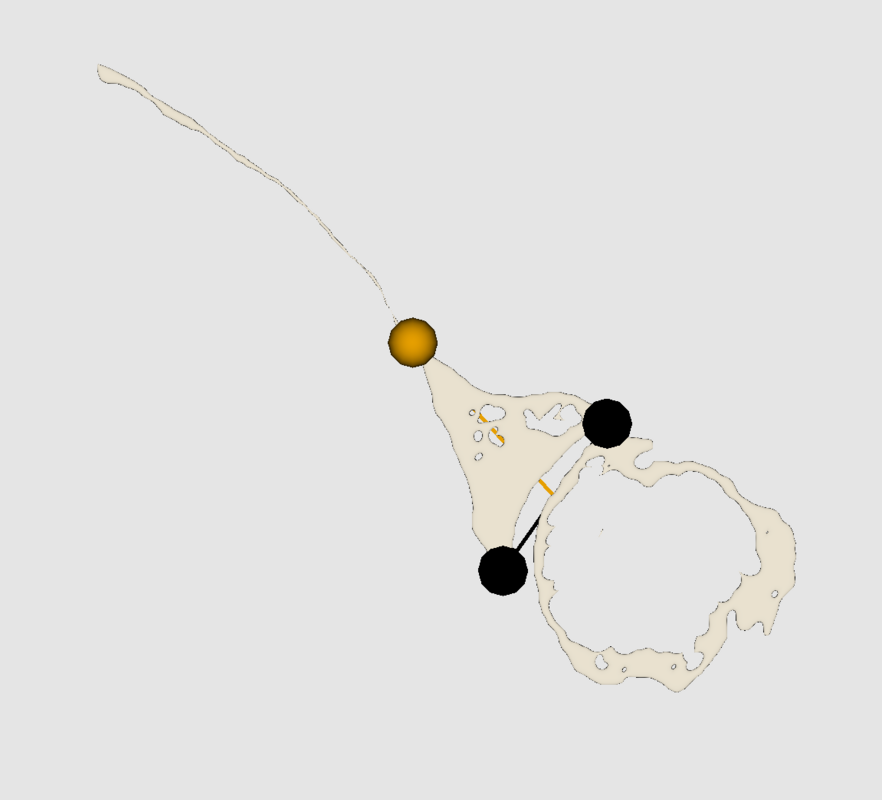
\includegraphics[width=\linewidth]{figures/vault_vis2D.png}
			\caption{\label{fig:visvault2D}Vault Method Axial Slice}
		\end{subfigure}	
	\end{center}
	\caption{\label{fig:visualisations}Visualisations of the 2 plane, Friedman and Vault methods and of new axial slice plane used for corrected Friedman method. Additional visualisations of the axial slices of the Friedman and vault methods to show point selection. By default, \sksglenoid uses the colour blind friendly palette defined by Wong\cite{bang2011}}
\end{figure}

For the Friedman and vault method 3 points were chosen to form 2 lines. Both require the same two points at the edges of the glenoid fossa anteriorly and posteriorly (black points on \ref{fig:visfried} and \ref{fig:visvault}). For the Friedman method the third point was selected at the tip of the scapula, while for the vault method it was at the tip of the scapular vault. The point selection is done on a 2D axial slice (see \ref{fig:visfried2D} and \ref{fig:visvault2D}). Therefore, slice choice is important and in this case was selected as the axial slice at which the coracoid process is no longer visible. The Friedman line was formed with the medial point on the scapula and the midpoint between the glenoid fossa points, while the vault line was formed with the tip of the scapular vault and the same midpoint. The second line was formed across the glenoid fossa in both methods. The version was then calculated as the angle between the two lines. 

The corrected Friedman method requires the same anatomical landmark points as the conventional Friedman method, but on a corrected axial plane. This plane (blue plane in \ref{fig:visplanes}) should be perpendicular to the scapular plane which is formed by the same 3 points as the scapular plane for the two-plane method (black plane in \ref{fig:visplanes}). The new transverse scapular plane (blue plane in \ref{fig:viscorrfried}) was used to generate a new 2D image slice on which the same conventional Friedman landmark points were selected.

\subsection{Software Implementation with SciKit-Surgery}
%these commands might work on some systems if you have -shell-escape set but I couldn't get it working on overleaf
%\immediate\write18{wget https://glenoidplanefitting.readthedocs.io/en/latest/_images/graphviz-f4a0d46f29de525cf2512540ebd2f3e3f3356594.png}
%\input|"wget https://glenoidplanefitting.readthedocs.io/en/latest/_images/graphviz-f4a0d46f29de525cf2512540ebd2f3e3f3356594.png"
\sksglenoid is built on top of the \sksurgery \cite{PMID:32436132} libraries which enabled
rapid development and future deployment into a clinically useable application. 
Development was kick started using the \sksurgery Python Template \cite{doel_tom_2022_5879146} enabling the bulk of the development and testing to be performed during a 10 week summer internship with minimal prior experience of Python or software development. Use of the Python Template encourages good software development practice \cite{schroeder2004software} from the outset of the development process. \sksurgery also includes template libraries for C++ projects \cite{dowrick2021cmakecatchtemplate}.

\sksurgery is made up of multiple Python libraries that can be assembled into
varied applications for research in image guided surgery. Some current examples 
of \sksurgeryns's use include clinical
guidance systems \cite{schneider2020comparison}, research platforms for registration \cite{thompson2021fiducial} and ultrasound simulators \cite{thompson2020snappysonic}.
Figure \ref{fig:deps} shows the immediate dependencies of \sksglenoidns. The most significant dependencies are NumPy\cite{2020NumPy-Array} which is used for the version calculation, and {VTK}\cite{Schroeder:1998:VTO:272980} which is used for visualising the results. SciKit-SurgeryCore provides configuration helpers for the user interface. SciKit-SurgeryVTK provides some helpful loaders and shape primitives, but it may be useful to remove this dependency in the future as it would significantly simplify the dependency graph.

\begin{figure}
        \begin{center}
                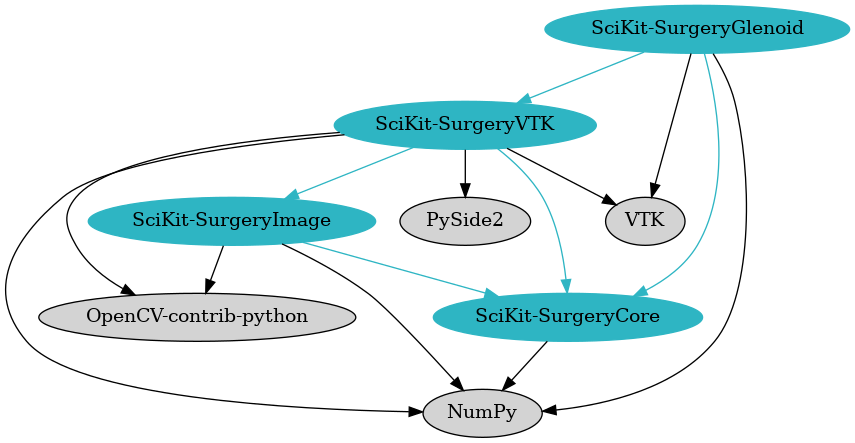
\includegraphics[width=0.6\linewidth]{figures/dep_graph.png}
                        \caption{\label{fig:deps}The dependency graph for SciKit-SurgeryGlenoid. SciKit-Surgery dependencies are shown in blue, whilst 3rd party dependencies are shown in grey.}
        \end{center}
\end{figure}

\subsection{Experimental Validation}
\label{sec:exp_methods}
We tested the performance of \sksglenoid on 10 anonymised {CT} scans from patients 
eligible for shoulder replacement surgery. For each {CT} scan we performed segmentation 
and landmark annotation using 3DSlicer \cite{Kikinis2014} and processed
the resulting 
segmentation using \sksglenoidns. 

Statistical analysis was performed using GraphPad Prism software version 8.0 for
Mac \footnote{GraphPad Software, San Diego, CA, USA}. The mean and standard deviation of 
each method was calculated and compared. Our current clinical practice uses planning 
software from {DJO} Surgical \cite{djosurgical}, so we compared the results from 
\sksglenoid with the results from the {DJO} Surgical software. 
Pearson’s correlation coefficient was 
determined between the commercial software and each method. 
A repeated measures ANOVA was performed to determine any significant differences
in version measurements between the methods. Significance level for all analyses was set at 0.05.

